\subsection{Complete six-method FLUX interventions}\label{app:flux22}
The FLUX cat intervention study contains 18 checkpoints and 396 evaluations, covering all six methods at their largest tested budgets. LR maximizes mean step-700 validation DINO, with ties favoring lower LR. Interventions use the final checkpoints and jointly replace all 80 adapted matrices.

\begin{table}[!htbp]
\caption{FLUX intervention operating points selected by mean validation DINO. Parameters are in millions. Displacements pool all adapted matrices before normalization. All edits act jointly on 80 matrices.}
\label{tab:flux22-protocol}
\begin{center}
\setlength{\tabcolsep}{3pt}
\begin{tabular*}{\linewidth}{@{\extracolsep{\fill}}lrrrrrr@{}}\toprule
Method & Capacity & LR & Params. (M) & $100d_W$ & $100d_S$ & $100d_S/d_W$\\\midrule
\textcolor{LoRAColor}{LoRA} & 32 & $5\times10^{-5}$ & $\result{fx22_lora_params}$ & $\result{fx22_lora_trained_dW_mean}_{\pm \result{fx22_lora_trained_dW_sd}}$ & $\result{fx22_lora_trained_dS_mean}_{\pm \result{fx22_lora_trained_dS_sd}}$ & $\result{fx22_lora_trained_ratio_mean}_{\pm \result{fx22_lora_trained_ratio_sd}}$\\
\textcolor{OFTColor}{OFT} & 256 & $1\times10^{-4}$ & $\result{fx22_oft_params}$ & $\result{fx22_oft_trained_dW_mean}_{\pm \result{fx22_oft_trained_dW_sd}}$ & $\result{fx22_oft_trained_dS_mean}_{\pm \result{fx22_oft_trained_dS_sd}}$ & $\result{fx22_oft_trained_ratio_mean}_{\pm \result{fx22_oft_trained_ratio_sd}}$\\
\textcolor{DoRAColor}{DoRA} & 32 & $1\times10^{-4}$ & $\result{fx22_dora_params}$ & $\result{fx22_dora_trained_dW_mean}_{\pm \result{fx22_dora_trained_dW_sd}}$ & $\result{fx22_dora_trained_dS_mean}_{\pm \result{fx22_dora_trained_dS_sd}}$ & $\result{fx22_dora_trained_ratio_mean}_{\pm \result{fx22_dora_trained_ratio_sd}}$\\
\textcolor{PiSSAColor}{PiSSA} & 32 & $5\times10^{-5}$ & $\result{fx22_pissa_params}$ & $\result{fx22_pissa_trained_dW_mean}_{\pm \result{fx22_pissa_trained_dW_sd}}$ & $\result{fx22_pissa_trained_dS_mean}_{\pm \result{fx22_pissa_trained_dS_sd}}$ & $\result{fx22_pissa_trained_ratio_mean}_{\pm \result{fx22_pissa_trained_ratio_sd}}$\\
\textcolor{MiLoRAColor}{MiLoRA} & 32 & $1\times10^{-4}$ & $\result{fx22_milora_params}$ & $\result{fx22_milora_trained_dW_mean}_{\pm \result{fx22_milora_trained_dW_sd}}$ & $\result{fx22_milora_trained_dS_mean}_{\pm \result{fx22_milora_trained_dS_sd}}$ & $\result{fx22_milora_trained_ratio_mean}_{\pm \result{fx22_milora_trained_ratio_sd}}$\\
\textcolor{HRAColor}{HRA} & 124 & $3\times10^{-4}$ & $\result{fx22_hra_params}$ & $\result{fx22_hra_trained_dW_mean}_{\pm \result{fx22_hra_trained_dW_sd}}$ & $\result{fx22_hra_trained_dS_mean}_{\pm \result{fx22_hra_trained_dS_sd}}$ & $\result{fx22_hra_trained_ratio_mean}_{\pm \result{fx22_hra_trained_ratio_sd}}$\\
\bottomrule\end{tabular*}
\end{center}
\end{table}
\FloatBarrier
\begin{table}[!htbp]
\caption{FLUX value-restoration controls. DINO scores and paired differences are multiplied by 100. The last column compares restoration with reconstruction through the same SVD/storage path.}
\label{tab:flux22-controls}
\begin{center}
\setlength{\tabcolsep}{3pt}
\begin{tabular*}{\linewidth}{@{\extracolsep{\fill}}lrrrrr@{}}\toprule
Method & Trained & Reconstructed & Restored & Values only & $\Delta$ vs. recon.\\\midrule
\textcolor{LoRAColor}{LoRA} & $\result{fx22_lora_trained_dino_mean}_{\pm \result{fx22_lora_trained_dino_sd}}$ & $\result{fx22_lora_reconstruct_dino_mean}_{\pm \result{fx22_lora_reconstruct_dino_sd}}$ & $\result{fx22_lora_restore_dino_mean}_{\pm \result{fx22_lora_restore_dino_sd}}$ & $\result{fx22_lora_spectrum_only_dino_mean}_{\pm \result{fx22_lora_spectrum_only_dino_sd}}$ & $\result{fx22_lora_restore_dino_vs_reconstruct_mean}_{\pm \result{fx22_lora_restore_dino_vs_reconstruct_sd}}$\\
\textcolor{OFTColor}{OFT} & $\result{fx22_oft_trained_dino_mean}_{\pm \result{fx22_oft_trained_dino_sd}}$ & $\result{fx22_oft_reconstruct_dino_mean}_{\pm \result{fx22_oft_reconstruct_dino_sd}}$ & $\result{fx22_oft_restore_dino_mean}_{\pm \result{fx22_oft_restore_dino_sd}}$ & $\result{fx22_oft_spectrum_only_dino_mean}_{\pm \result{fx22_oft_spectrum_only_dino_sd}}$ & $\result{fx22_oft_restore_dino_vs_reconstruct_mean}_{\pm \result{fx22_oft_restore_dino_vs_reconstruct_sd}}$\\
\textcolor{DoRAColor}{DoRA} & $\result{fx22_dora_trained_dino_mean}_{\pm \result{fx22_dora_trained_dino_sd}}$ & $\result{fx22_dora_reconstruct_dino_mean}_{\pm \result{fx22_dora_reconstruct_dino_sd}}$ & $\result{fx22_dora_restore_dino_mean}_{\pm \result{fx22_dora_restore_dino_sd}}$ & $\result{fx22_dora_spectrum_only_dino_mean}_{\pm \result{fx22_dora_spectrum_only_dino_sd}}$ & $\result{fx22_dora_restore_dino_vs_reconstruct_mean}_{\pm \result{fx22_dora_restore_dino_vs_reconstruct_sd}}$\\
\textcolor{PiSSAColor}{PiSSA} & $\result{fx22_pissa_trained_dino_mean}_{\pm \result{fx22_pissa_trained_dino_sd}}$ & $\result{fx22_pissa_reconstruct_dino_mean}_{\pm \result{fx22_pissa_reconstruct_dino_sd}}$ & $\result{fx22_pissa_restore_dino_mean}_{\pm \result{fx22_pissa_restore_dino_sd}}$ & $\result{fx22_pissa_spectrum_only_dino_mean}_{\pm \result{fx22_pissa_spectrum_only_dino_sd}}$ & $\result{fx22_pissa_restore_dino_vs_reconstruct_mean}_{\pm \result{fx22_pissa_restore_dino_vs_reconstruct_sd}}$\\
\textcolor{MiLoRAColor}{MiLoRA} & $\result{fx22_milora_trained_dino_mean}_{\pm \result{fx22_milora_trained_dino_sd}}$ & $\result{fx22_milora_reconstruct_dino_mean}_{\pm \result{fx22_milora_reconstruct_dino_sd}}$ & $\result{fx22_milora_restore_dino_mean}_{\pm \result{fx22_milora_restore_dino_sd}}$ & $\result{fx22_milora_spectrum_only_dino_mean}_{\pm \result{fx22_milora_spectrum_only_dino_sd}}$ & $\result{fx22_milora_restore_dino_vs_reconstruct_mean}_{\pm \result{fx22_milora_restore_dino_vs_reconstruct_sd}}$\\
\textcolor{HRAColor}{HRA} & $\result{fx22_hra_trained_dino_mean}_{\pm \result{fx22_hra_trained_dino_sd}}$ & $\result{fx22_hra_reconstruct_dino_mean}_{\pm \result{fx22_hra_reconstruct_dino_sd}}$ & $\result{fx22_hra_restore_dino_mean}_{\pm \result{fx22_hra_restore_dino_sd}}$ & $\result{fx22_hra_spectrum_only_dino_mean}_{\pm \result{fx22_hra_spectrum_only_dino_sd}}$ & $\result{fx22_hra_restore_dino_vs_reconstruct_mean}_{\pm \result{fx22_hra_restore_dino_vs_reconstruct_sd}}$\\
\bottomrule\end{tabular*}
\end{center}
\end{table}
\FloatBarrier


\paragraph{Evaluation and numerical references.}
The BF16 evaluator generates $512\times512$ images with 20 sampling steps and guidance 3.5. Test DINO averages four held-out image/prompt pairs with three generation repeats. The drift bank has five class prompts and five general prompts, with general drift and CLIP using the latter. Drift is $(1-\text{DINO cosine})/2$ relative to base-generated images. 

Every change is paired within a checkpoint before computing the mean and sample SD. Component effects use the same-run merged trained model, restoration controls use reconstruction through the same SVD/storage path, and comparisons of retained task performance use full value restoration. Same-run references account for this difference. All 396 evaluations succeed, with every restored matrix matched and within the recorded numerical tolerance.

\begin{figure}[!htbp]\centering
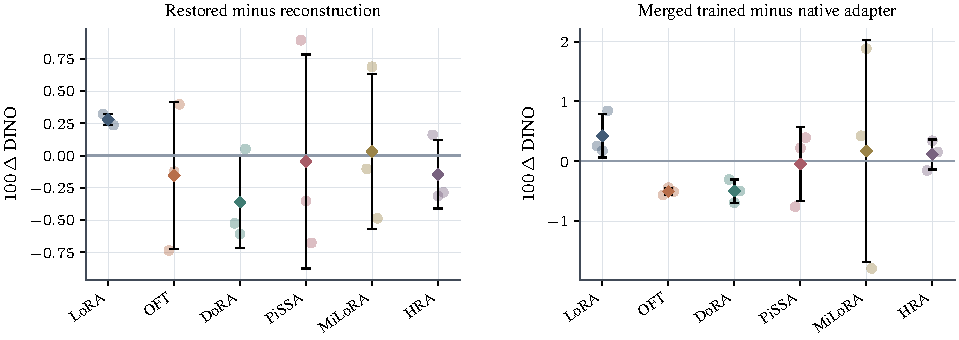
\includegraphics[width=.98\linewidth]{figures/flux22_controls.pdf}
\caption{FLUX numerical controls. The left panel compares value restoration with reconstruction. The right panel compares the same-run merged trained model with the earlier native-adapter evaluation. Diamonds and bars show means and sample SDs, with faint points for individual checkpoints. Differences are in DINO scores $\times100$.}
\label{fig:flux22-controls}
\end{figure}
\FloatBarrier

\paragraph{Values and adapted bases.}
Value restoration nearly preserves fidelity for every method, whereas learned values on pretrained singular bases yield near-base scores (\Cref{tab:flux22-controls}). This extends the main restoration finding to diffusion and points to the adapted bases as the principal source of task gains. Spectral displacement concentrates in PiSSA's dominant components and MiLoRA's trailing components (\Cref{fig:flux22-spectrum}). 

\begin{figure}[!htbp]\centering
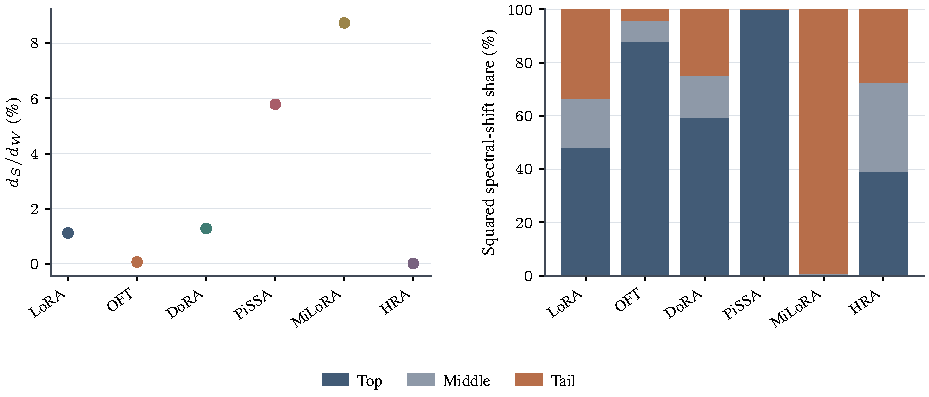
\includegraphics[width=.98\linewidth]{figures/flux22_spectrum.pdf}
\caption{FLUX spectral displacement. The left panel shows the pooled spectral-to-weight displacement ratio with sample SDs. The right panel shows mean shares of squared singular-value displacement across component groups, with boundaries adjusted to pretrained spectral gaps. Shares are computed from all measured spectral vectors.}
\label{fig:flux22-spectrum}
\end{figure}
\FloatBarrier

\subsection{Task performance and forgetting across spectral components}
The dominant, intermediate and trailing component groups are approximate thirds adjusted to nearby pretrained spectral gaps. Restore and keep operations replace complete rank-one contributions, using pretrained singular values as in \cref{eq:band-restore}. The measured response includes these interactions between components.

Restoring dominant components reduces general drift in every checkpoint and gives the largest mean reduction for each method. It gives the largest individual reduction in 17 of 18 checkpoints. MiLoRA seed zero has a slightly larger trailing-component response. Class-prompt drift also decreases in every checkpoint, with dominant restoration giving the largest reduction. Both drift measures therefore support the recurring dominant-component response. CLIP responses differ, with LoRA's mean general-prompt alignment decreasing. OFT gains fidelity on average but loses fidelity in one checkpoint.

Keeping only the adapted dominant components nearly preserves mean fidelity for LoRA, DoRA and PiSSA. LoRA and DoRA reduce general drift in every checkpoint, whereas PiSSA retains essentially all its drift. These responses show that similar retained task performance can accompany different retention outcomes. Fidelity losses vary across seeds, including a larger DoRA loss. We report DINO changes directly and use the 1 pp sufficiency rule only for language accuracy. OFT/HRA have greater trained drift than PiSSA in these selected settings.

\begin{figure}[!htbp]\centering
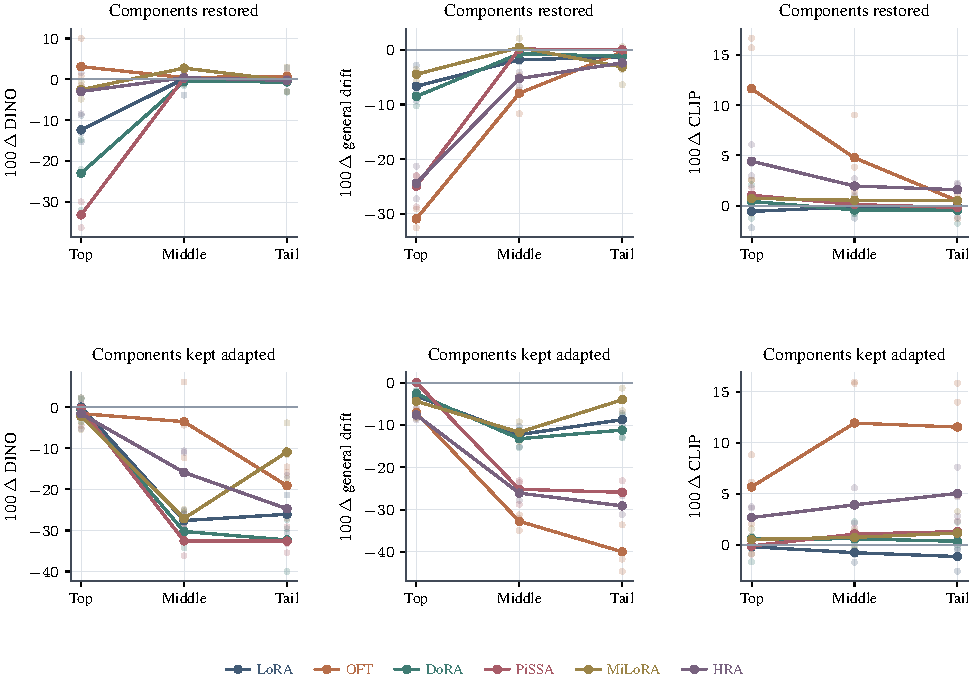
\includegraphics[width=.98\linewidth]{figures/flux22_bands.pdf}
\caption{FLUX component-restoration responses. The top row restores the named component group, and the bottom row keeps only that adapted group. All changes use the same-run trained model. Lines show method means and faint points show individual checkpoints.} 
\label{fig:flux22-bands}
\end{figure}

\FloatBarrier

\paragraph{Summary.}
The FLUX results extend the singular-value restoration and dominant-component forgetting findings to image personalization.
\FloatBarrier
